\documentclass{standalone}
\usepackage{tikz,upgreek}
\usepackage{ctex,siunitx}
\setCJKmainfont{Noto Serif CJK SC}
\usepackage{tkz-euclide}
\usepackage{amsmath}
\usetikzlibrary{patterns, calc,3d}
\usetikzlibrary {decorations.pathmorphing,decorations.pathreplacing,decorations.shapes}
\begin{document}
\small
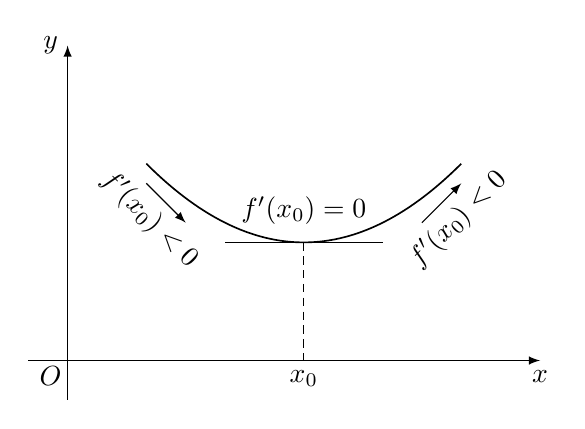
\begin{tikzpicture}[>=latex,scale=1.0]
  \draw[->](-0.5,0)--(6,0)node[below]{$x$};
  \draw[->](0,-0.5)--(0,4)node[left]{$y$};
  \draw[semithick,samples=200,domain=1:5]plot(\x,{0.25*\x*\x-1.5*\x+3.75});
  \draw[densely dashed](3,1.5)--(3,0)node[below]{$x_0$};
  \draw(2,1.5)--(4,1.5)node[midway,above=3pt]{$f'(x_0)=0$};
  \node at (0,0)[below left,inner sep=2pt]{$O$};
  \draw[<-](1.5,1.75)--++(-0.5,0.5)node[midway,sloped,below]{$f'(x_0)<0$};
  \draw[->](4.5,1.75)--++(0.5,0.5)node[midway,sloped,below]{$f'(x_0)<0$};
\end{tikzpicture}
\end{document}